\chapter{Experimental Setup}

Our approach is based upon the popular and influential Hiero system \cite{chiang07} which uses a synchronous context free grammar (SCFG) to model translation. 
This translation system uses only a single non-terminal symbol and therefore the system is inherently stateless. 
However, we know that using a richer set of non-terminals can greatly improve translation, as evidenced by the improvments obtained by SAMT system \cite{samt} which augments a Hiero-style SCFG model with syntactic labels.
This is best explained in terms of the generalisation capability: a single category grammar can create all manner of string-pairs, the majority of which are nonsensical and agrammatical, while a model with syntactic categories inherently limits the sets of string pairs to those which are grammatical (largely).
This can be seen from the following example rules, showing how rules can be combined to arrive at ungrammatical string pairs.
\begin{align}
X &\rightarrow \langle \mbox{does not}~X, \mbox{ne}~X~\mbox{pas} \rangle \label{eq:nepas}\\
X &\rightarrow \langle \mbox{cat}, \mbox{chat} \rangle \label{eq:chat} \\
X &\Rightarrow^{\ref{eq:nepas},\ref{eq:chat}} \langle \mbox{does not cat}, \mbox{ne cat pas} \rangle
\nonumber
\end{align}
If the non-terminals in the above rules were replaced with, e.g., parts-of-speech, such that rule \ref{eq:nepas} required a verb instead of an X in its right hand side, and the rule \ref{eq:chat} rewrote a noun, then this ungrammatical string pair would no longer be licenced.

As such, the single-category model licenses all manner of word-salad output, thus relying on the language model to salvage a coherent sentence from these options.
In contrast, the set of translation options for the grammar with syntactic labels is much smaller and more coherent, and thus the language model has less heavy lifting to do.
This setting plays well to the strengths of a n-gram language model which can accurately model local coherence but is unable to model global sentence-level effects (which are modelled by the syntactic translation model). 
%In addition, a treebank parser and an n-gram language model have different strengths -- the parser can ensure more global grammatical coherence but over-generalises at the lexical level, while the n-gram model does the opposite.

The central aim of the project was to induce automatically a rich translation grammar to realise some of the performance gains resulting from the use of linguistic grammars, but without using linguistic resources such as treebank parsers.
This allows our approach to be more easily ported to work for translating a variety of languages, rather than being constrained to just translating into languages with good syntactic resources (typically English).

\section{Distributional Hypothesis}

Underlying most models of grammar induction is the distributional hypothesis. This theory states that
``words that occur in the same contexts tend to have similar meaning'' \cite{harris:54}. Although phrased in terms of semantics, the distributional hypothesis applies equally to syntax, that is, words that can be substituted for one another most often share the same syntactic category (in general, semantics implies syntax). This is evidenced by the wide-spread use of the substitution test in theories of syntax to determine the constituency and syntactic category of a word or phrase.

The majority of work on monolingual grammar induction has used some notion of context to inform the induced categories. This is best seen in the work of Alex Clark who uses the context surrounding a phrase to determine its category, and in Dan Klein's work, which uses context to determine constituency. In this project we follow the lead of these earlier works on monolingual grammar induction by using context to inform our clustering of words and phrases, such that words that appear in similar contexts are assigned to the same cluster. We expect that this clustering should bear a strong resemblance to the underlying syntax and, to some extent, the semantics of the language, and therefore improve translation accuracy.

Our bilingual translation setting differs from the earlier monolingual settings in which most grammar induction research has been performed. We seek to label a broad range of n-grams (so-called phrases) as supplied from the phrase extraction process. These n-grams will be both constituents and non-constituents. The use of non-constituent translation units has been shown consistently to outperform systems which use only constituents in terms of translation quality. For this reason how grammar induction system must be able to infer useful syntactic categories for these non-constituent n-grams.

\section{Clustering Configuration}

It still remains to define what we mean by context. Well we could choose the entire sentence or even document in which the phrase appears, we adopt a more local definition of context. We use a window of one or two words preceding the phrase and one or two words following. This local context is still highly informative about the syntactic role of the phrase, but given its small size we expect to observe the same context many times in a small corpus. That is, the sparsity of the data should no lo

It still remains to define what we mean by context. Well we could choose the entire sentence or even document in which the phrase appears, we adopt a more local definition of context. We use a window of one or two words preceding the phrase and one or two words following. This local context is still highly informative about the syntactic role of the phrase, but given its small size we expect to observe the same context many times in a small corpus. That is, the sparsity of the data should no longer be a serious problem, as it would be for full sentences or example.

The input to the clustering system are bilingual phrases in their bilingual contexts, as extracted using the standard phrase-based grammar extraction pipeline. However we choose to primarily perform monolingual clustering by discarding one side of the data, typically the source. Focusing our attention on the target side of the corpus replicates the configuration which is known to work best for syntactic translation. The target-side syntax is more informative than source-side syntax, it better models the target language and also avoids an errorful projection step onto the target (due to the grammars of the two languages not being isomorphic). On the flip side, source side syntax could be more useful in pruning the beam search for decoding, where we can use the source parse to prune away improbable items before translating into the target language. We will determine experimentally whether the effects of better pruning versus better modelling target grammar are more important for translation.
nger be a serious problem, as it would be for full sentences or example.

The input to the clustering system are bilingual phrases in their bilingual contexts, as extracted using the standard phrase-based grammar extraction pipeline. This is illustrated in Figure~\ref{fig:extraction}. Instead of using the bilingual data directly, we choose to primarily perform monolingual clustering by discarding one side of the data, typically the source. Focusing our attention on the target side of the corpus replicates the configuration which is known to work best for syntactic translation. The target-side syntax is more informative than source-side syntax, as it better models the target language, thus better informing reordering and lexical selection. Target-side syntax avoids an errorful projection step onto the target, due to the grammars of the two languages rarely being even approximately isomorphic. On the flip side, source side syntax could be more useful in pruning the beam search for decoding, where we can use the source parse to prune away improbable items before translating into the target language. We will determine experimentally whether the effects of better pruning versus better modelling target grammar are more important for translation.

\begin{CJK}{UTF8}{gbsn}
\begin{figure}
% input: 今天 有 棒球 比赛 吗 ? ||| are there any baseball games today ? ||| 1-0 1-1 1-2 2-3 3-4 0-5 4-6 5-6
% from btec/split.zh-en.al line 26
\centering
\subfigure[Example word-aligned sentence pair]{\hfill 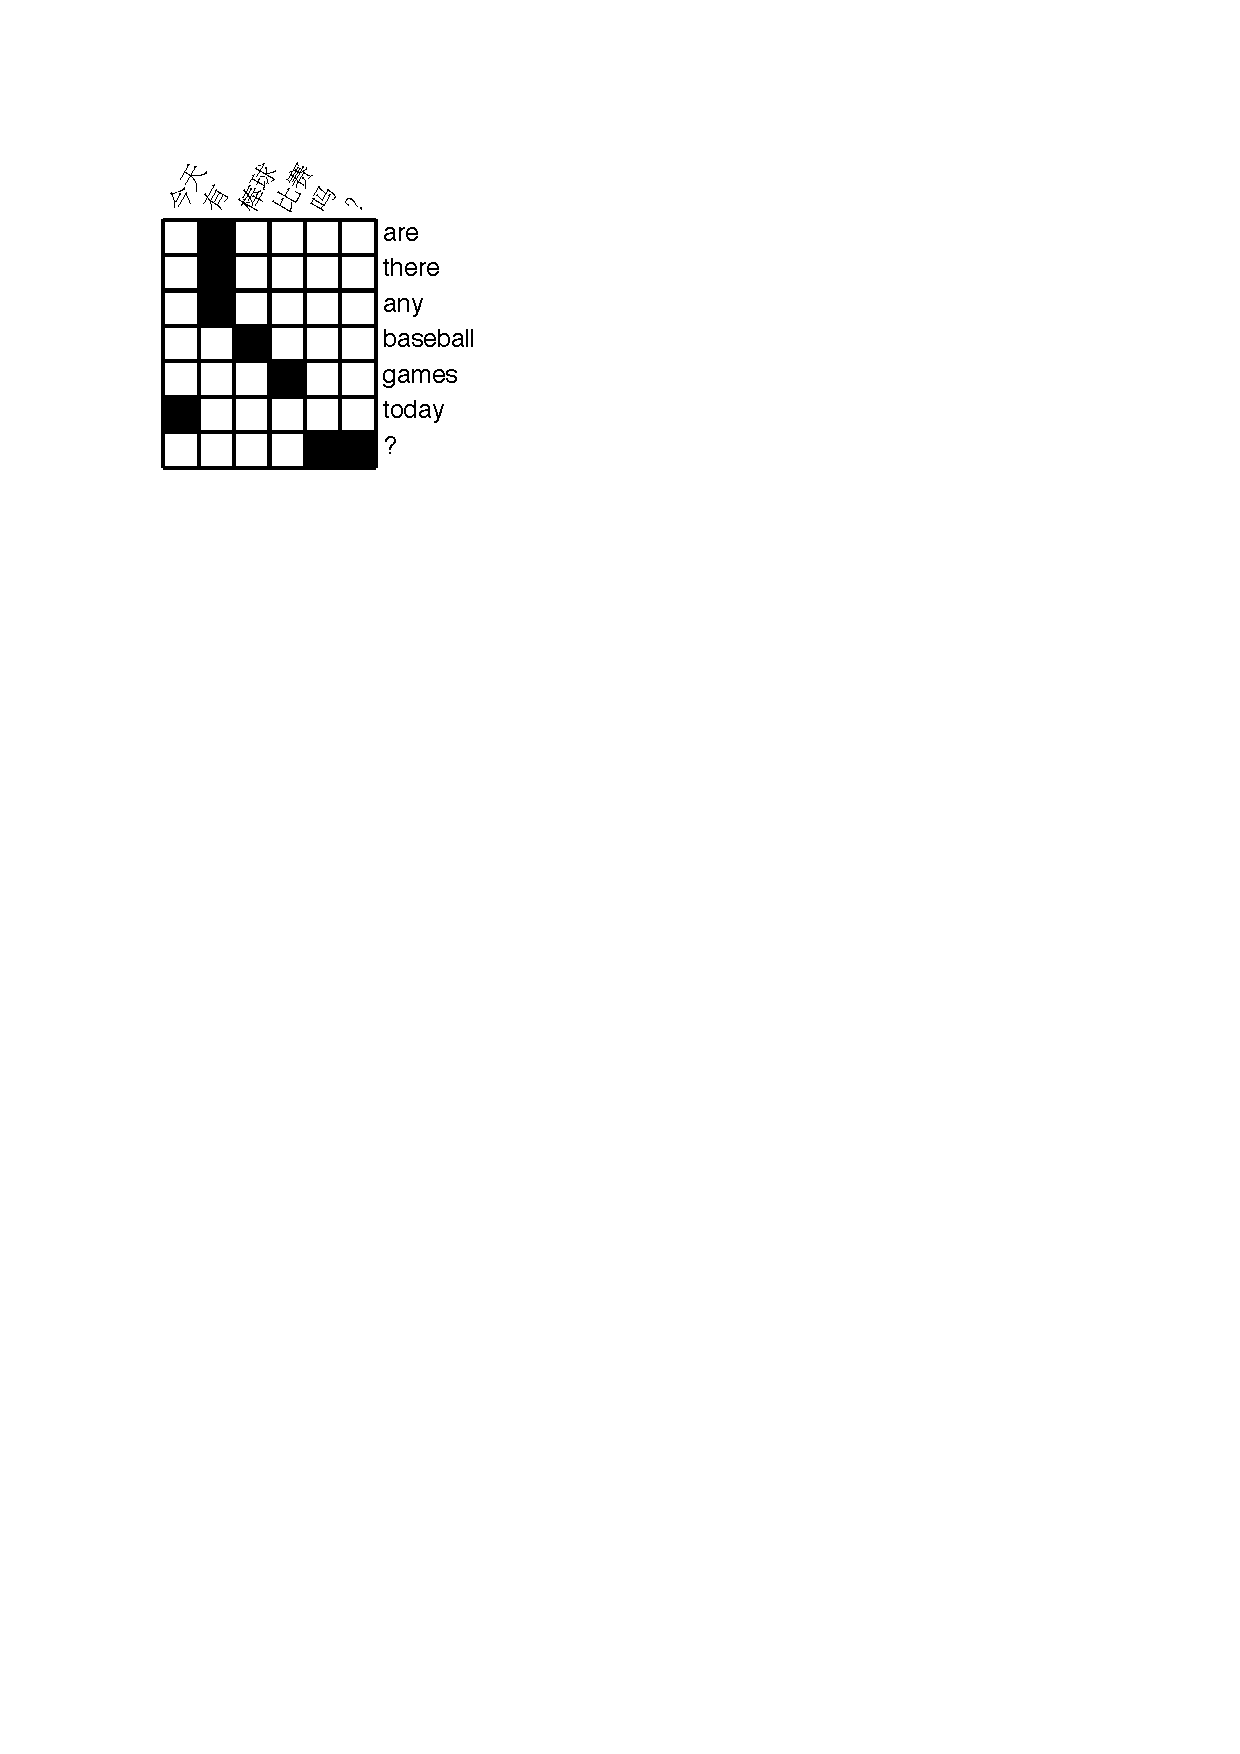
\includegraphics{align} \hfill}

\subfigure[Some bilingual phrases and contexts extracted from (a)]{
\centering
\begin{tabular}{rcl}
\toprule
$<$s$>$ $<$s$>$ & are there any baseball games today & ? $<$/s$>$ \\
$<$s$>$ $<$s$>$ & 今天 有 棒球 比赛 & 吗 ? \\ 
\midrule
baseball games & today & ? $<$/s$>$ \\
$<$s$>$ $<$s$>$ & 今天 & 有 棒球 \\
\midrule
$<$s$>$ $<$s$>$ & are there any & baseball games \\
$<$s$>$ 今天 & 有 & 棒球 比赛 \\
\midrule
any baseball & games & today ? \\
有 棒球 & 比赛 & 吗 ? \\
\bottomrule
\end{tabular}}
\caption{Example showing how a sentence pair gives rise to bilingual phrases and their contexts. These serve as input to the clusterer, typically by discarding the source side and processing the target.}
\label{fig:extraction}
\end{figure}
\end{CJK}

In addition to the choice of source versus target language, we also consider the choice of lexical units. Our default option is to use words, but we also consider using automatically induced parts of speech in their stead. To do this we replace the words in the corpus with their corresponding word classes, and then run the extraction heuristics to obtain the phrase context graphs over parts-of-speech. This improves the density of the counts, because many different phrases and contexts will share the same part-of-speech sequence. In addition the part-of-speech induction algorithm uses a different mechanism for learning the labelling -- namely, a form of hidden Markov model with a hard-clustering constraint -- and therefore would be expected to present complementary information to our methods of indepedently clustering each instance based solely on its context. For these reason we expect that using word classes rather than words will improve the results of our clustering methods. There is one caveat: errors in the word-classes will artifically conflate many disparate syntactic categories. This is not a huge problem for the contexts, where it will resemble noise in the data, however for phrases this is more of a problem. All of our models make the assumption that phrases are assigned very few different cluster labels, but when using word class sequences for phrases this will no longer be valid. For this reason we have also experimented with a conglomerate representation where the contexts are represented as word-classes but the phrases are composed of words. This means that we obtain the expected improvements in data sparsity, but without also conflating phrases which are not syntactically or semantically identical.

The set of phrases and contacts are aggregated over the corpus, and are then collated into a file consisting of phrases, context and their occurrence counts. We refer to this structure as the phrase -- context graph, as illustrated in Figure \ref{fig:bipartite}. This is a bipartite graph with nodes for each phrase type and context type, and edges for instances of a phrase occurring in a given context.  The graph forms the input to the clustering algorithm, which labels the edges with cluster indices.  In the example, we expect that the clustering will produce two different clusters for nouns (the sub-graph to the right of `deal') and for verbs (the sub-graph to the left). This clustering maximises internal connectivity within each sub-graph while minimising external connectivity between the two sub-graphs. In other words, outgoing edges from phrases and contexts are largely assigned the same cluster label. 

\begin{figure}
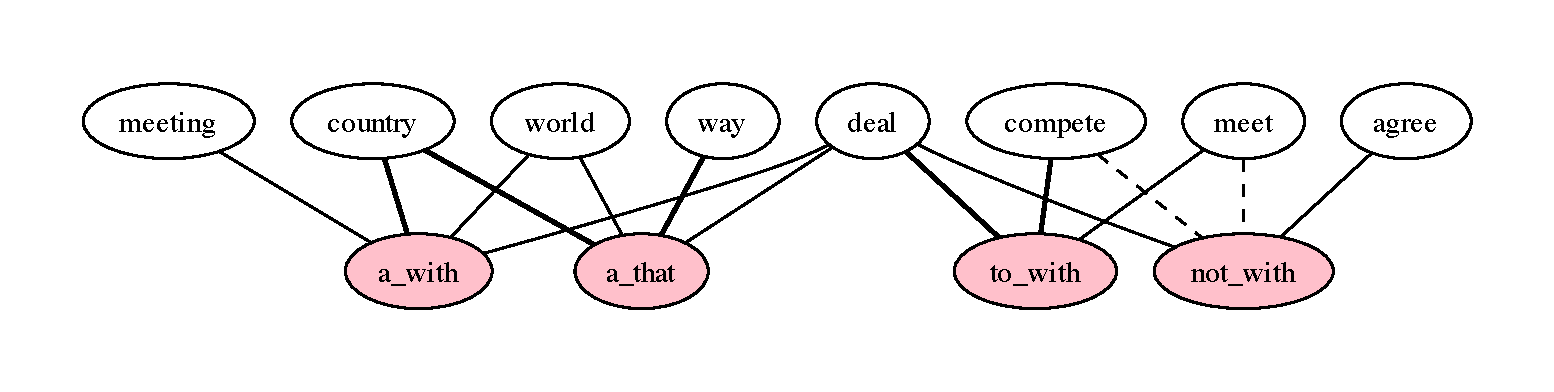
\includegraphics[width=\textwidth]{deal}
\caption{Example of a phrase-context graph, centered around `deal'. Phrases are shown as unshaded nodes and contexts are shaded in pink. Contexts include the left and right word surrounding the phrase, with an underscore denoting the gap for the phrase. Edges specify that phrase appears in a given context, and the edge weight denotes the occurence count.}
\label{fig:bipartite}
\end{figure}

The notation used in the remainder of the paper for describing the clustering models and their inputs and outputs is given in Table~\ref{tab:notation}.

\begin{table}
\begin{tabular}{cp{.7\textwidth}}
\toprule
  symbol & meaning \\
\midrule
  $\mathbf{p} = (p_1, \ldots, p_n)$ & a phrase (n-gram) of word tokens \\
  $\mathbf{c} = (\ldots, c_{-2}, c_{-1}, c_1 c_2, \ldots)$ & a context of immediate words surrounding a phrase, with the index signifying the distance to the left (negative indices) or right (positive indices) of the phrase \\
  $e = (p, c)$  & a edge denoting a phrase, $p$, occuring in context $c$ \\
  $z$ & label assigned to an edge, denoting the cluster or non-terminal assigned to the phrase in context \\
  $K$ & number of clusters, $z \in \{1,2, \ldots, K\}$ \\
  $P$ & set of unique phrases \\
  $C$ & set of unique contexts \\
  $C_p$ & set of contexts in which $p$ has occurred \\
  $P_c$ & set of phrases occuring in context $c$ \\
\bottomrule
\end{tabular}
\caption{Notation used throughout this paper.}
\label{tab:notation}
\end{table}

\section{Pipeline}

Brief overview of the pipeline, including phrase-extraction.

\section{Data sets}

\section{Evaluation}

Given an induced clustering, we run the pipeline to completion to produce translations for our test set. We then compare these translations with human authored reference translations in order to evaluate the quality. We use the standard metric, blue, to measure the quality of the output translations. However as an alternative metric we consider an intrinsic evaluation of the clustering by comparing the induced labels against linguistic categories. That is, without running the decoder to create translations. This saves considerable time and also gives us an alternative view as to the quality of the clustering. We now describe each of these evaluation metrics in the following section.

\subsubsection{BLEU}


\subsubsection{Conditional Entropy}

The second evaluation metric measures the similarity between the induced cluster labels and the syntactic categories predicted by a treebank-trained parser. This metric is considerably cheaper to evaluate than BLEU as it does not require a decoding pass, but instead works directly on the clustering output. Our objective is to maximise the quality of translation, and we trust BLEU to do this more directly than this instrinsic metric. However, we expect there to be interesting information in this metric, and the potential to short-cut the evaluation thus improving the turn-around time for experimental evaluation. 

We measure the conditional entropy of the ``gold-standard'' categories for each phrase in context given the cluster labelling. For the gold-standard we use the predicted constituent categories from a tree-bank parser on the target side (English). Many phrases are not constituents, and therefore the parser output does not include their category; We exclude such phrases from the evaluation. The conditional entropy measures the amount of surprise at seeing the gold standard categories given that we know the clusters. If the cluster labels closely resemble the syntax, then there will be little surprise and the entropy will be low. If however the clusters do not match the syntax at all entropy will be very high. The conditional entropy is formulated as follows:
\[ H(S|Z) = \sum_{s,z} p(s,z) \log \frac{p(z)}{p(s,z)} \]
where $s$ are the constituent labels as output from a parser, $p(s,z)$ is the frequency of $s$ and $z$ labelling the same edge and $p(z)$ is the frequency of label $z$. If the clustering maps perfectly onto the syntax, then $z$ will always coocur with $s$ and the $\log$ term will vanish, resulting in a conditional entropy of zero. This metric can be gamed by using a separate category for every edge, and thereby still realising a perfect mapping but without any intelligent clustering at all. This degeneracy is not relevant for our models as we limit ourselves to small label sets, typically using $K = 25$ which is considerably fewer than the hundred or so syntactic categories in a treebank parser. 

%%% Local Variables: 
%%% mode: latex
%%% TeX-master: "report"
%%% End: 
